\subsection{Leistungsverhalten bei Spannungsabfall}\label{subsec:LeistungSpannungabfall}
Bei diesem Versuch wird das Verhalten des Controllers bei einem Spannungsabfall untersucht. Dabei wurde sowohl die Leistung der ASM (Abbildung \ref{fig:Spannungsabfall} rechts) als auch der Strom des Controllers (Abbildung \ref{fig:Spannungsabfall} links) in Abhängigkeit zur Spannung des Controllers gemessen. Der Drehmoment-Sollwert wurde während des gesamten Versuchs konstant auf dem Nennmoment gehalten. Die Versuchsbedingungen können der Tabelle \ref{tab:Spannungsabfall} entnommen werden.

\begin{table}[H]
	\centering
	\begin{tabular}{C{4cm} C{4cm} C{3cm}} 
		\multicolumn{3}{c}{\textbf{Versuchsbedingungen}} \\
		{Messgrösse}& {Bedingung} & {Wert}\\ \hline\hline 
		Spannung (DC)   & nachgeregelt &   96 V     \\
		Strom (DC)   & gemessen &   1.6-107 A     \\
		Leistung (AC)   & gemessen &   0-5666 W    \\
		Drehzahl   & konstant &   1200 RPM    \\
		Drehmoment-Sollwert   & variiert &   0-50 Nm    \\
		Motor-Temperatur   & gemessen &   40-100 °C    \\
		Controller-Temperatur   & vernachlässigt &   -    \\
	\end{tabular}
	\caption{Versuchsbedingungen Steuerkennlinie}\label{tab:Spannungsabfall}
\end{table}



Dieser Versuch wurde zuerst mit 1500 RPM (blaue Punkte) und danach nochmals mit 2000 RPM (rote Punkte) durchgeführt. 

\begin{figure}[H]
	\centering
	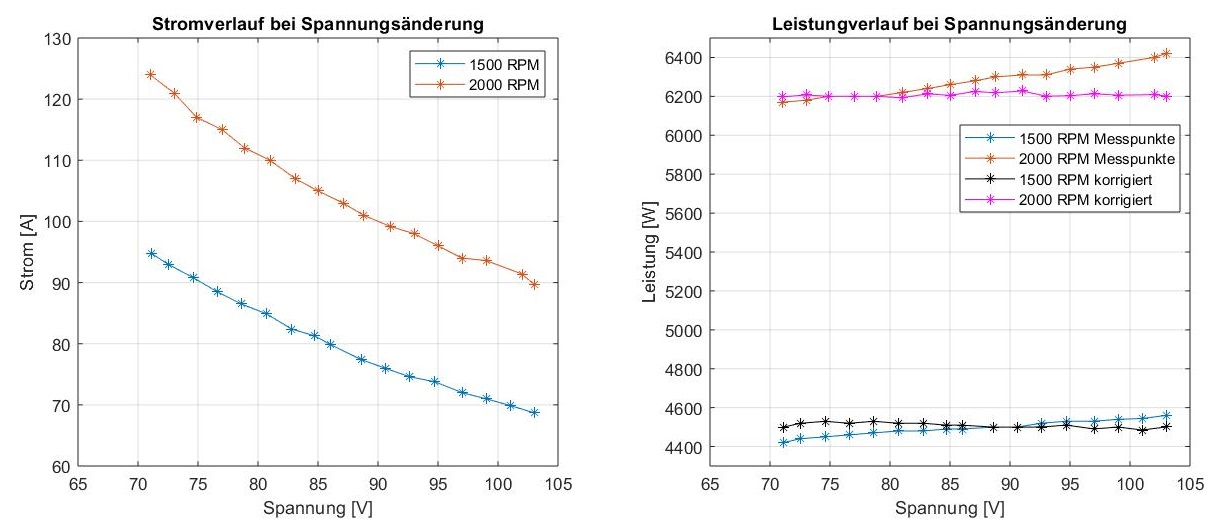
\includegraphics[width=1\linewidth]{Spannungsversuch.jpg}
	\caption{Leistungs- und Stromverlauf bei Spannungsabfall}\label{fig:Spannungsabfall}
\end{figure}

Aus diesem Versuch ist ersichtlich, dass der Controller bei einem Spannungsabfall und konstantem Drehmomentsollwert die Leistung nachregelt indem der Strom erhöht wird. Während die Spannung um 32\% abfällt, nimmt der Strom um ca. 28\% zu. Dabei verhält sich die Stromzunahme linear zum Spannungsabfall. Die Leistung nimmt dabei lediglich um ca. 4\% ab.

Dadurch kann der Schluss gezogen werden, dass der Spannungsabfall keinen grossen Einfluss auf die Leistung hat. Durch die erhöhte thermische Belastung bei grösseren Ströme ist eine möglichst grosse Spannung jedoch erstrebenswert.